\chapter{Schroedinger equation in 2d}

Schrodinger equation in 2d:
\begin{equation}
\left[ -\frac{1}{2}\nabla^2 + V(x,y) \right] \psi(x,y) = E\,\psi(x,y)
\end{equation}
%
where $\nabla^2$ is the Laplacian operator:
\begin{equation}
\nabla^2 = \frac{\partial^2}{\partial x^2} + \frac{\partial^2}{\partial y^2}
\end{equation}


\section{Finite difference grid in 2d}

\begin{juliacode}
struct FD2dGrid
    Npoints::Int64
    Nx::Int64
    Ny::Int64
    hx::Float64
    hy::Float64
    dA::Float64
    x::Array{Float64,1}
    y::Array{Float64,1}
    r::Array{Float64,2}
    idx_ip2xy::Array{Int64,2}
    idx_xy2ip::Array{Int64,2}
end
\end{juliacode}


\begin{juliacode}
function FD2dGrid( x_domain, Nx, y_domain, Ny )
    x, hx = init_FD1d_grid(x_domain, Nx)
    y, hy = init_FD1d_grid(y_domain, Ny)
    dA = hx*hy
    Npoints = Nx*Ny
    r = zeros(2,Npoints)
    ip = 0
    idx_ip2xy = zeros(Int64,2,Npoints)
    idx_xy2ip = zeros(Int64,Nx,Ny)
    for j in 1:Ny
        for i in 1:Nx
            ip = ip + 1
            r[1,ip] = x[i]
            r[2,ip] = y[j]
            idx_ip2xy[1,ip] = i
            idx_ip2xy[2,ip] = j
            idx_xy2ip[i,j] = ip
        end
    end
    return FD2dGrid(Npoints, Nx, Ny, hx, hy, dA, x, y, r, idx_ip2xy, idx_xy2ip) 
end
\end{juliacode}

\section{Laplacian operator}

Given second derivative matrix in $x$, $\mathbb{D}^{(2)}_{x}$,
$y$ direction, $\mathbb{D}^{(2)}_{x}$,
we can construct finite difference representation of the Laplacian operator
$\mathbb{L}$ by using
%
\begin{equation}
\mathbb{L} = \mathbb{D}^{(2)}_{x} \otimes \mathbb{I}_{y} +
\mathbb{I}_{x} \otimes \mathbb{D}^{(2)}_{y}
\end{equation}
%
where $\otimes$ is Kronecker product.
In Julia, we can use the function \jlinline{kron} to form the Kronecker product
between two matrices \jlinline{A} and \jlinline{B} as \jlinline{kron(A,B)}.

\begin{juliacode}
function build_nabla2_matrix( fdgrid::FD2dGrid; func_1d=build_D2_matrix_3pt )
    Nx = fdgrid.Nx
    hx = fdgrid.hx
    Ny = fdgrid.Ny
    hy = fdgrid.hy
    
    D2x = func_1d(Nx, hx)
    D2y = func_1d(Ny, hy)

    ∇2 = kron(D2x, speye(Ny)) + kron(speye(Nx), D2y)
    return ∇2
end
\end{juliacode}

Example to the approximation of 2nd derivative of 2d Gaussian function

\begin{figure}[H]
{\center
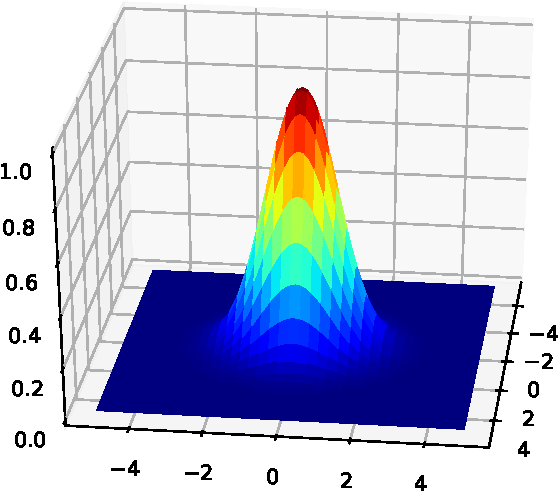
\includegraphics[width=0.45\textwidth]{codes/2d/IMG_gaussian2d.pdf}
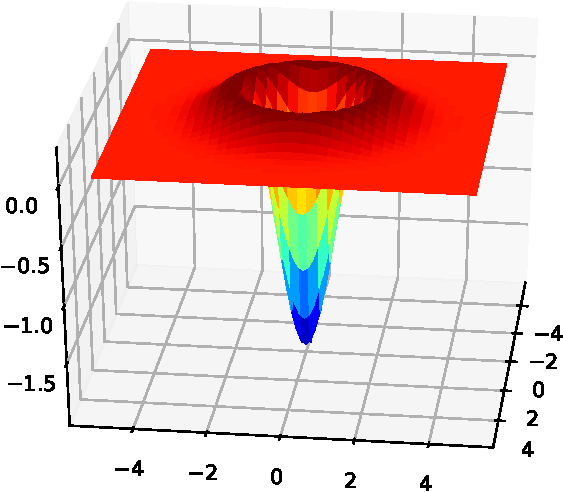
\includegraphics[width=0.45\textwidth]{codes/2d/IMG_d2_gaussian2d.pdf}
\par}
\caption{Two-dimensional Gaussian function and its finite difference
approximation of second derivative}
\end{figure}

\section{Iterative methods for eigenvalue problem}

The Hamiltonian matrix:
\begin{juliacode}
∇2 = build_nabla2_matrix( fdgrid, func_1d=build_D2_matrix_9pt )
Ham = -0.5*∇2 + spdiagm( 0 => Vpot )
\end{juliacode}

The Hamiltonian matrix size is large. The use \jlinline{eigen} method
to solve this eigenvalue problem is not practical.
We also do not need to solve for all eigenvalues.
We must resort to the
so called iterative methods.

